%
% chapter3.tex
%

\chapter{NVIDIA Bluefield-3}
\label{cha:design}
Die im Rahmen dieser Arbeit verwendete SmartNIC ist die von Nvidia im Jahre 2022 veröffentlichte Bluefield-3. Wie bereits am Namen der Karte zu erkennen ist, handelt es sich dabei um die dritte Generation von Netzwerkkarten, die zusätzlich zur netzwerkspezifischen Architektur noch einen allgemeinen ARM-Prozessor verbaut hat. Zusätzlich wird in einem späteren Abschnitt ein Überblick über das DOCA-Framework gegeben, welches von NVidia als einheitliche Programmierschnittstelle veröffentlicht wurde, um die Programmierung der Hardware von der jeweiligen Generation unabhängig zu machen.
\section{Entstehung}
Die Entwicklung der BlueField ist ein Produkt der letzten Dekade, in der ein immerwährend größeres Interesse an der Effizienzsteigerung von Rechenzentren entstanden ist. Energiesparende Systeme, die die selbe Leistung erreichen wie selbige Integration auf einem allgemeinen Prozessor, bieten für Systemintegratoren eine ausgezeichnete Möglichkeit, auch vor dem Hintergrund des Klimawandels energieoptimierte Systeme zu entwickeln.
\subsection{BlueField-1}
Die erste Generation der Bluefield-Hardware wurde im Jahre 2017 von Mellanox Technologies vorgestellt und bildet den ersten Eintrag in die Reihe der Bluefield-SmartNIC-Serie. Sie kombinierte erstmalig die ConnectX-5-Plattform mit einem ARM-basierten System-on-Chip. Die Idee dahinter war es, das Verhalten der Netzwerkplattform mittels User-Anwendungen beeinflussen zu können. Dazu wurde eine API zwischen der ConnectX und dem ARM-Prozessor entwickelt. Hierzu sei erwähnt, dass es sich bei der ConnectX-Plattform um eine bereits weit verbreitete und in viele Systeme integrierte Hardware handelte. Sie besaß bereits zum damaligen Zeitpunkt eine breite Anzahl von paketbasierten Operationen, mit deren Hilfe eine weitreichende Manipulation sowie Paket-Steering oder anderweitige Verwendungen ermöglicht wurden. Die BlueField-1 war mit einem ARM-A72 mit 4 Kernen und 8 Threads ausgestattet und besaß außerdem zwei QSFP28-Anschlüsse, welche bis zu 100 Gbps Durchsatz erreichen konnten. Die Zielgruppe der BlueField-Serie war von Anfang an der Enterprise-Markt sowie die zahlreichen größeren Rechenzentren, in denen Rechenoperationen ausgeführt werden, die auf mehreren Computern eines Clusters oder einer Clusterstruktur ausgeführt werden. Gerade in diesem Umfeld wird eine derartige Architektur von Interesse, da der Netzwerkverkehr so anwendungsspezifischer verteilt werden kann und somit die Effizienz eines Rechnerverbundes steigern kann. 
\begin{figure}
    \centering
    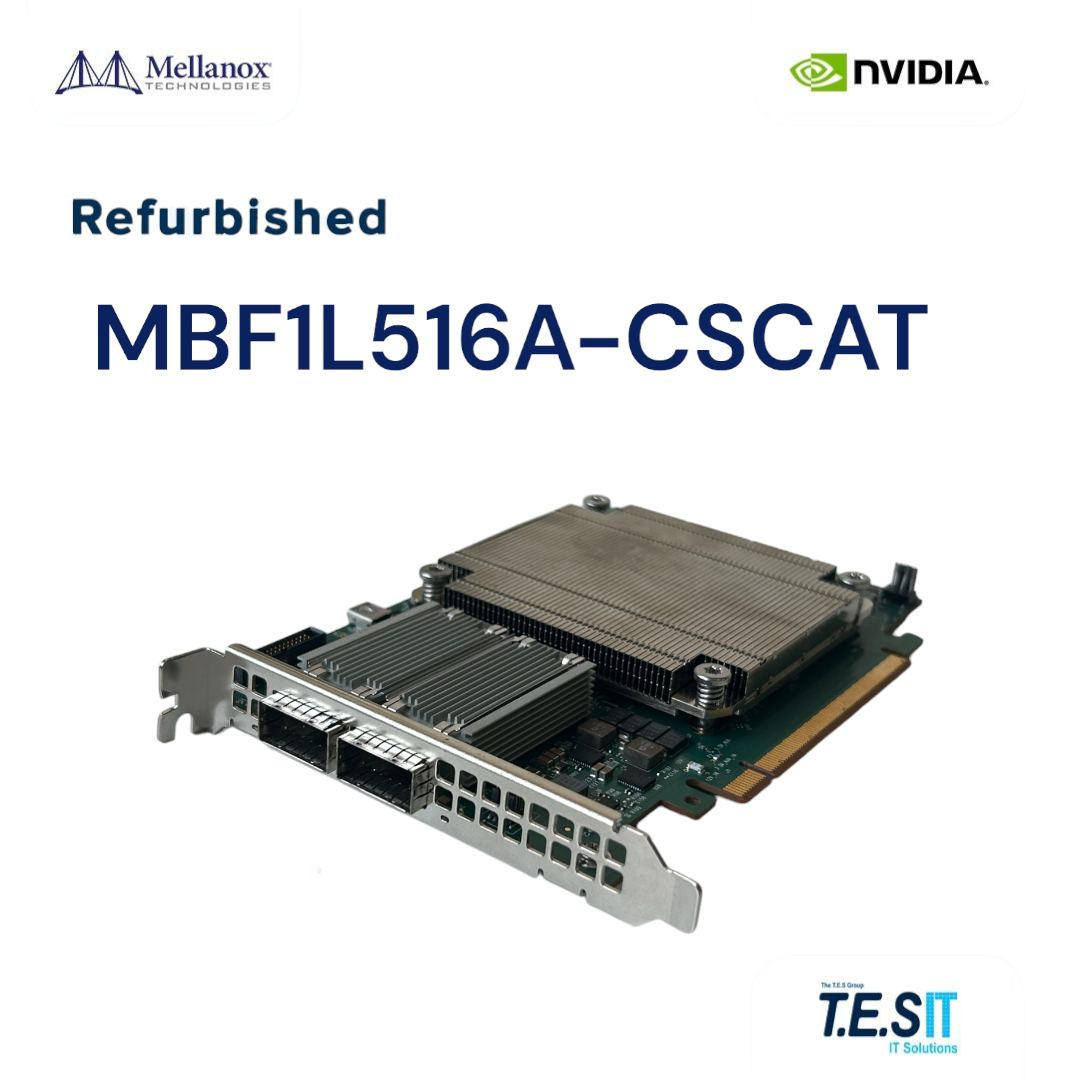
\includegraphics[width=0.65\linewidth]{images/s-l1600.png}
    \caption{BlueField-1 Karte}
    \label{fig:enter-label}
\end{figure}
\subsection{BlueField-2}
Nach der Übernahme von Mellanox durch den Chip-Hersteller NVIDIA im Jahre 2019 wurde das Projekt BlueField von NVIDIA nicht nur weitergeführt, sondern mit dem Aufkommen von vermehrten Machine Learning Workloads sogar das Marketing ausgebaut. So wurde die BlueField-2 im Jahre 2021 unter dem neuen Hersteller NVIDIA veröffentlicht und bot nun einen QSFP56, der laut eigenem Marketing-Material bis zu 200 Gbps erreichen sollte. Abermals kam der ARM A72 zum Einsatz, der erneut mit 4 Kernen und 8 Threads verbaut wurde. 
\subsection{BlueField-3}
Zuletzt wurde im Jahre 2022 die BlueField-3 veröffentlicht, die im Rahmen dieser Arbeit zur Verwendung kam. Erstmalig wurde nun der ARM-A78 mit 8 Kernen und somit 16 Threads verbaut. Die Arbeitsspeicherarchitektur nahm zusätzlich auch den Generationensprung von DDR4 auf DDR5 und verwendet so deutlich schnelleren Speichertakt als die vorherige Generation. Außerdem wurde erneut der Netzwerkanschluss aktualisiert und verwendet nun den QSFP112. Laut NVIDIA soll mit diesem Netzwerkverbund eine Line Rate von bis zu 400 Gbps erreicht werden. Dabei wird im Marketing-Material nicht explizit erwähnt, welche Paketgröße für besagten Durchsatz verwendet wurde. Erneut soll laut NVIDIA der Fokus der Hardware vermehrt auf dem Einsatz in Rechenzentren liegen, in denen größere Machine-Learning-Lasten laufen. Die BlueField-3 soll daraufhin die Rolle einer intelligenteren Paketverteilung einnehmen, wobei die Last der Lastverteilung nicht mehr auf dem Hostsystem bzw. dem entsprechenden Host-Prozessor liegen, sondern eben auf der Netzwerkkarte selbst. Außerdem sind eine Menge von weiteren speziellen hardwarebeschleunigten Hardwareeinheiten auf der neuesten Iteration der BlueField-Serie verbaut worden. Alle genannten Generationen BlueField werden per PCI-E Stecker in den Hostsystemen verbaut und verwenden so den aktuellsten PCI-E 5.0 Standard, der auf eine theoretische Maximalbandbreite von 32 Giga Transfer/s kommt. Somit soll eine ultraschnelle Schnittstelle zwischen Hostsystem und BlueField-3 erreicht werden.
\section{Architektur}
Um der Funktion einer intelligenten Netzwerkkarte nachzukommen, sind auf der BlueField diverse Hardwareeinheiten verbaut, die eine Reihe von Einsatzzwecken abdecken sollen. Dabei werden nicht alle angebotenen Funktionen auch tatsächlich von ASIC-Hardwareeinheiten übernommen, sondern werden teilweise komplette oder nur in bestimmten Pipeline-Abschnitten auf dem ARM Core ausgelagert, um dort einer weiteren Behandlung unterzogen zu werden. Von Hause aus werden folgende Beschleuniger und Funktionen angeboten.
\begin{figure}
    \centering
    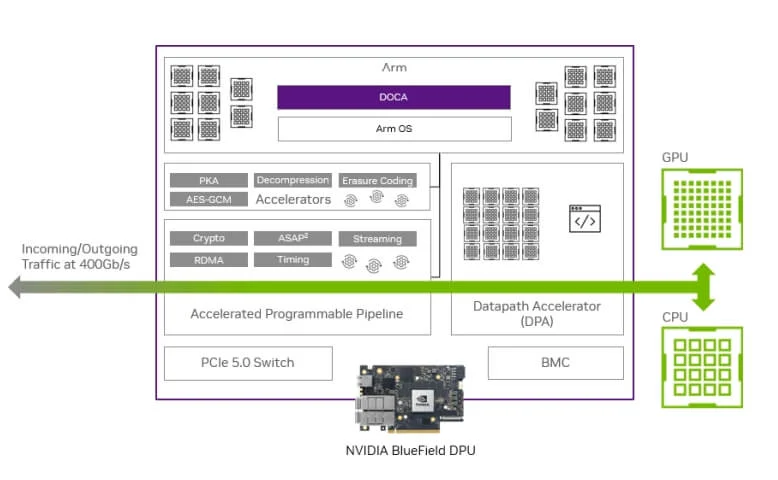
\includegraphics[width=1\linewidth]{images/nvda-bluefield-dpu.png}
    \caption{BlueField-3 Architektur}
    \label{fig:enter-label}
\end{figure}
\subsection{Hardwareeinheiten}
\subsubsection{PKA}
PKA steht für Public-Key-Acceleration

\subsubsection{Decompression}
\subsubsection{Erasure Coding}
\subsubsection{AES-GCM}
\subsubsection{Crypto}
\subsubsection{ASAP²}
\subsubsection{Streaming}
\subsubsection{RDMA}
\subsubsection{Timing}


\section{DOCA Framework}

